\documentclass[11pt]{beamer}
\usetheme{CambridgeUS}
\usepackage[utf8]{inputenc}
\usepackage{amsmath}
\usepackage{amsfonts}
\usepackage{amssymb}
\usepackage[
backend=biber,
style=alphabetic,
citestyle=authoryear
]{biblatex}
\usepackage{array}

% Footnote without number
\newcommand\blfootnote[1]{%
  \begingroup
  \renewcommand\thefootnote{}\footnote{#1}%
  \addtocounter{footnote}{-1}%
  \endgroup
}

\addbibresource{stats.bib}
\title[Bioestatística II] %optional
{Testando hipóteses com a variável padrão z}

\subtitle{CGF2046 - Bioestatística II}

\author[da Silva, Ricardo] % (optional, for multiple authors)
{R. ~R. ~da Silva\inst{1}}

\institute[FCFRP] % (optional)
{
  \inst{1}%
  Departamento de Ciências BioMoleculares\\
  Faculdade de Ciências Farmacêuticas

}

\date{\today} % (optional)

\titlegraphic{
\includegraphics[width=5.8cm]{figs/logo_final}} 

\begin{document}

%\begin{frame}
%\titlepage
%\end{frame}

%\begin{frame}
%\tableofcontents
%\end{frame}

\begin{frame}
\titlepage
\end{frame}

\begin{frame}
\label{contents}
\frametitle{Sumário}
\tableofcontents
\end{frame}

\setbeamercovered{transparent}
\begin{frame}
\frametitle{Objetivos de Aprendizado\footcite{carlson2017introduction}}
  Depois de assitir essa aula e fazer as atividades complementares, você será capaz de:
  \\~\\
  \begin{itemize}
  \uncover<1->{\item
    Escrever hipóteses nulas e alternativas usando parâmetros populacionais;}
  \uncover<2->{\item
    Calcular a z para uma média amostral;}
  \uncover<3->{\item
    Determinar se você deve ou não rejeitar a hipótese nula;}
   \uncover<4->{\item
    Calcular e interpretar o tamanho do efeito (d) de um estudo;}
   \uncover<5->{\item
    Identificar exemplos de erro Tipo I, erro Tipo II e poder estatístico;}
   \uncover<6->{\item
    Fornecer uma descrição detalhada de um valor p, valor crítico e valor calculado;}
  \end{itemize}
\end{frame}

\section{Introdução ao teste de hipótese}
\setbeamercovered{transparent}
\begin{frame}
\frametitle{Definições}
  No capítulo anterior, você aprendeu a
  \\~\\
  \begin{itemize}
  \uncover<1->{\item
    Calcular z para uma média amostral;}
  \uncover<2->{\item
    Localizar essa média amostral dentro de uma distribuição de médias amostrais;}
  \uncover<3->{\item
     Determinar a probabilidade dessa média amostral ocorrer devido ao erro de amostragem.}
  \end{itemize}
  \uncover<3->{Essas habilidades permitem testar hipóteses.}
\end{frame}

\setbeamercovered{transparent}
\begin{frame}
\frametitle{Teste de hipótese com z para uma média amostral (unicaudal)}

\textbf{Exemplo:} Suponhamos que uma professora redesenhe seu curso de história para que os alunos façam testes frequentes antes de fazer os exames.

\begin{itemize}
\item
  Nota média histórica para todos os alunos antes de exames frequentes (\(\mu = 75, \sigma = 10\));
\item
  Depois de um semestre usando esses questionários, a nota média no exame final dos 25 alunos do seu curso foi \(\bar{x} = 80\);
\end{itemize}

Com o teste de hipóteses, você pode determinar se a amostra de alunos que respondem aos testes frequentes teve pontuação "significativamente" melhor do que a dos alunos anteriores.

\end{frame}

\setbeamercovered{transparent}
\begin{frame}
\frametitle{Teste de hipótese com z para uma média amostral (unicaudal)}

Os questionários frequentes ajudaram?\\~\\

A média amostral de 80 é numericamente maior do que a média populacional de 75.\\~\\

O desvio entre a média amostral de 80 e a média populacional de 75 é provável ou improvável de ter ocorrido devido a erro amostral?\\~\\

Esses novos conceitos serão descritos em uma série de seis etapas.

\end{frame}

\setbeamercovered{transparent}
\begin{frame}
\frametitle{Etapa 1: examinar as variáveis para avaliar suposições estatísticas}

Todos os testes de hipóteses são baseados em suposições específicas e, se essas suposições forem violadas, esses testes podem produzir resultados enganosos.\\~\\
Os quatro pressupostos básicos são:

\begin{enumerate}
\item independência dos dados;
\item medição apropriada das variáveis para análise;
\item normalidade das distribuições;
\item homogeneidade da variância.
\end{enumerate}

\end{frame}

\setbeamercovered{transparent}
\begin{frame}
\frametitle{Etapa 1: examinar as variáveis para avaliar suposições estatísticas}

Os quatro pressupostos básicos são:

\begin{enumerate}
\item \textbf{independência dos dados:} a pontuação de cada participante dentro de uma condição é independente das pontuações de todos os outros;
\item \textbf{medição apropriada:} variável independente (VI) \(\Rightarrow\) identifica grupos diferentes, variável dependente (VD) \(\Rightarrow\) medida em uma escala númerica quantitativa;
\item \textbf{normalidade das distribuições:} distribuição das médias amostrais para cada condição deve ter uma forma normal;
\item \textbf{homogeneidade da variância:} variâncias em cada condição do estudo são semelhantes.
\end{enumerate}

\end{frame}

\setbeamercovered{transparent}
\begin{frame}
\frametitle{Etapa 2: expor as hipóteses nulas e de pesquisa simbolicamente e verbalmente}

Neste exemplo, o professor prevê que questionários frequentes aumentarão as pontuações dos testes. Embora a hipótese de pesquisa preveja que os questionários aumentarão os resultados dos testes, é possível que os questionários não funcionem. Esta segunda possibilidade é chamada de hipótese nula e é sempre o oposto da hipótese de pesquisa.

\begin{center}
\begin{tabular}{ m{2cm}|m{2cm}|m{3cm}|m{3cm} } 
 \hline
 Tipo de Hipótese & Simbólico & Vebal & Diferença entre médias amostral e populacional\\
  \hline
 Hipótese nula & $\mu_{quiz}=75;$ & Com questiónario notas $\approx$ 75 & Erro amostral \\ 
 Hipótese de pesquisa & $\mu_{quiz}>75.$ & Com questiónario notas $>$ 75 & Intervenção melhora resultados  \\ 
 \hline
 \hline
\end{tabular}
\end{center}

\end{frame}

\setbeamercovered{transparent}
\begin{frame}
\frametitle{Etapa 2: expor as hipóteses nulas e de pesquisa simbolicamente e verbalmente}
A notação simbólica do nulo e das hipóteses de pesquisa pode ser um pouco confusa. Porque estamos tentando determinar se $\mu_{quiz} > 75$, e já sabemos que $\bar{x} = 80$ e $\mu = 75$? \\~\\
É importante observar que o subscrito "quiz" em $\mu_{quiz} > 75$ refere-se àqueles que fazem testes frequentes antes do teste.\\~\\

Não sabemos qual seria a pontuação média do teste se toda a população de alunos respondesse aos testes frequentes antes da prova (ou seja, não sabemos o $\mu_{quiz}$).

Hipóteses: 
\[H_0: \mu_{quiz}=75;\] 
\[H_a: \mu_{quiz}>75.\]

\end{frame}

\setbeamercovered{transparent}
\begin{frame}
\frametitle{Passo 3: Definir a Região Crítica}
A região crítica é a coleção de todos os valores de z que são tão raros se o nulo for verdadeiro que, se qualquer um desses valores de z ocorrer, sugere que a hipótese nula é provavelmente falsa.
\begin{center}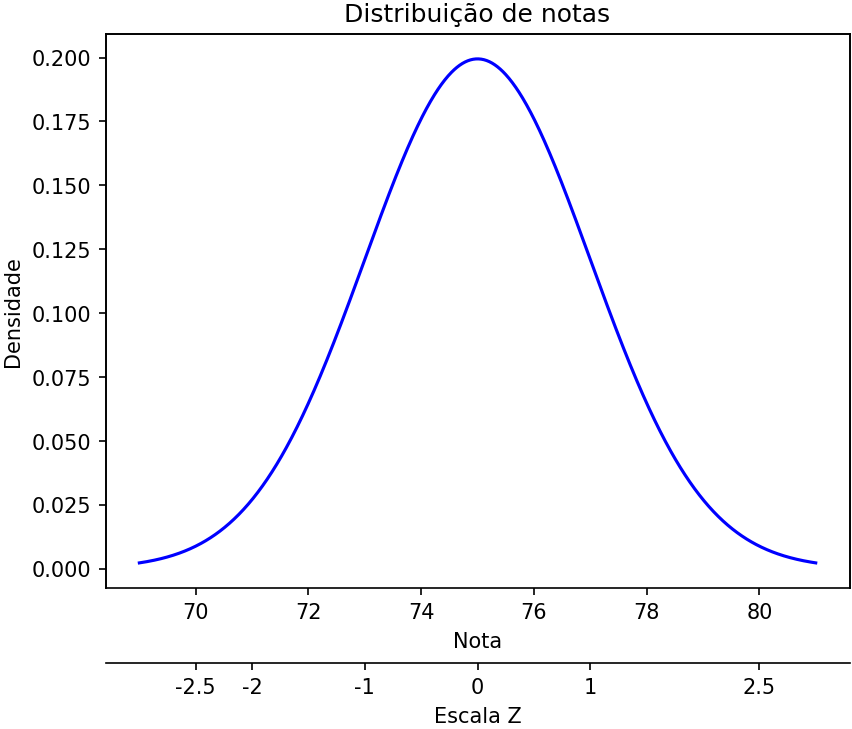
\includegraphics[width=0.6\linewidth]{figs/two_xticks_under} \end{center}

\end{frame}

\begin{frame}
\frametitle{Passo 3: Definir a Região Crítica}
\begin{columns}
\begin{column}{0.5\textwidth}
   A curva normal padrão e os valores de z\\~\\
   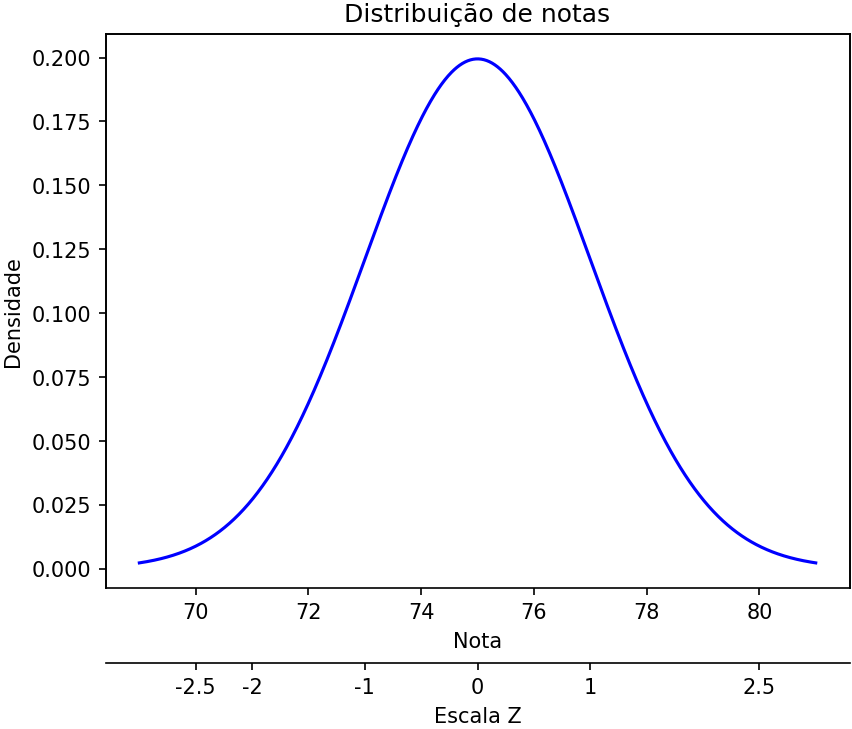
\includegraphics[width=1\linewidth]{figs/two_xticks_under}
\end{column}
\begin{column}{0.5\textwidth}  %%<--- here
   \begin{itemize}
   \item Se a hipótese nula for verdadeira, você esperaria um valor de z próximo a 0;
   \item Se a hipótese nula não for verdadeira, você esperaria um valor de z distante de 0.
   \end{itemize}
\end{column}
\end{columns}
\end{frame}

\setbeamercovered{transparent}
\begin{frame}
\frametitle{Média de dados brutos}

Divide-se a soma de todos os dados pelo número total deles:

\[
\bar{x}_{obs} = \frac{x_1 + x_2 + \cdots + x_n}{n} = \frac{\sum_{i=1}^n
x_i}{n}.
\]
\begin{center}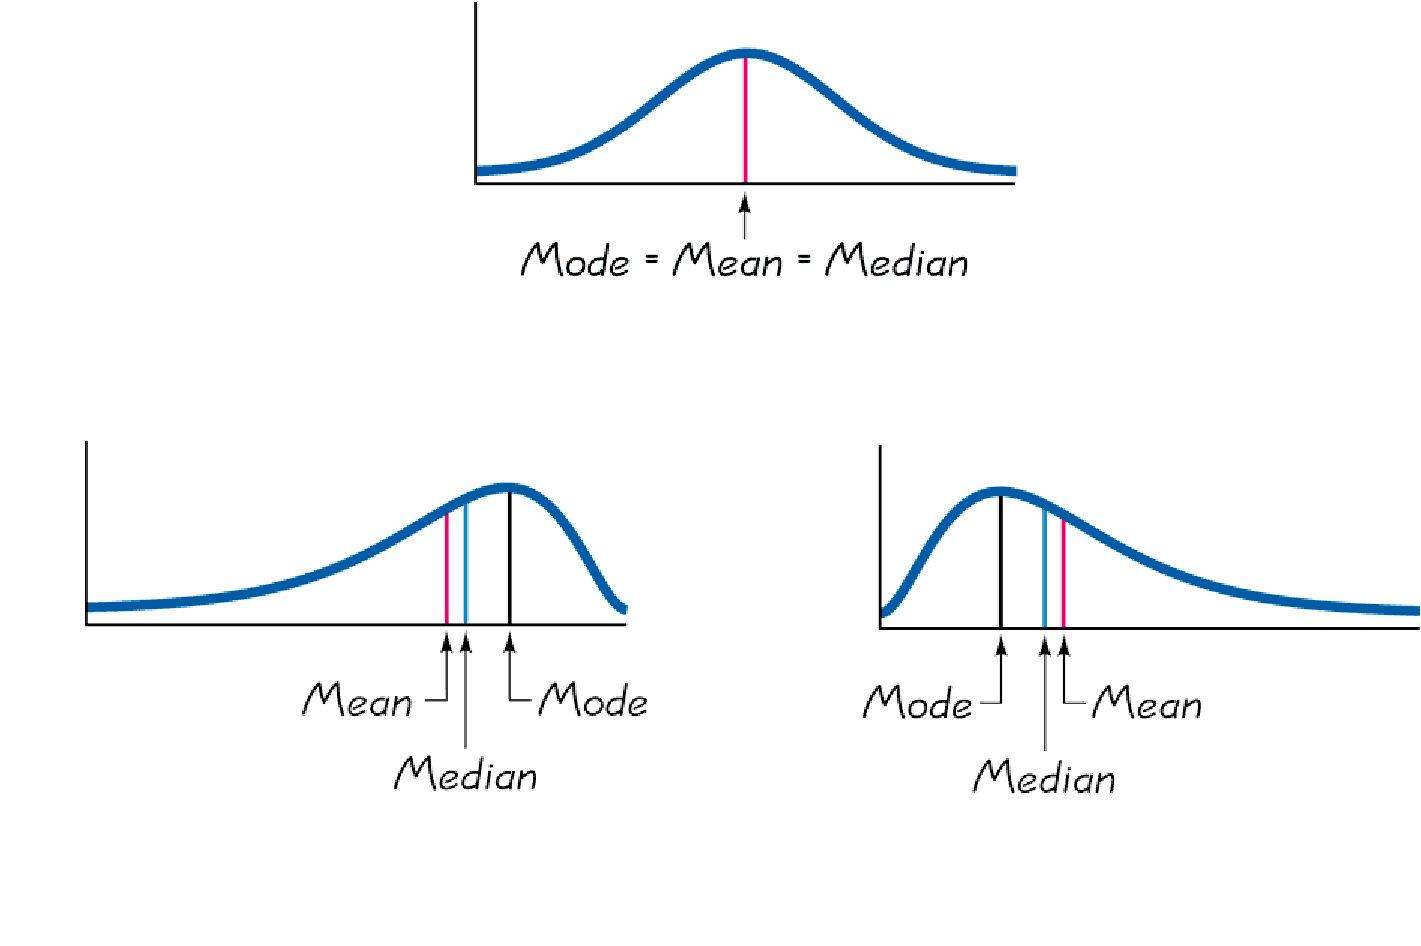
\includegraphics[width=0.8\linewidth]{figs/medidas-crop} \end{center}
\end{frame}

\setbeamercovered{transparent}
\begin{frame}
\frametitle{Variância e desvio-padrão de um conjunto de dados}

Uma alternativa melhor é usar a \textbf{soma dos quadrados dos desvios},
que dá origem à \textbf{variância} de um conjunto de dados \[
var_{obs} = \frac{1}{n}\sum_{i=1}^n (x_i - \bar{x}_{obs})^2
\] Para manter a mesma unidade de medida dos dados originais, definimos
o \textbf{desvio padrão} como \[
dp_{obs} = \sqrt{var_{obs}}
\] Uma expressão alternativa da variância (mais fácil de calcular) é \[
var_{obs} = \frac{1}{n}\sum_{i=1}^n x_i^2 - \bar{x}_{obs}^2
\]
\end{frame}


\section{Distribuição Amostral}
\setbeamercovered{transparent}
\begin{frame}
\frametitle{Intuição para distribuições amostrais}
Uma distribuição de médias amostrais é a população de todas as médias amostrais aleatórias possíveis para um estudo realizado com um determinado tamanho de amostra.\\~\\
População exemplo de quatro valores: \[10, 12, 14, 16\]

\end{frame}

\setbeamercovered{transparent}
\begin{frame}
\frametitle{Exemplo}
Distribuição de médias amostrais para a população de quatro valores e um tamanho de amostra de 2
\begin{center}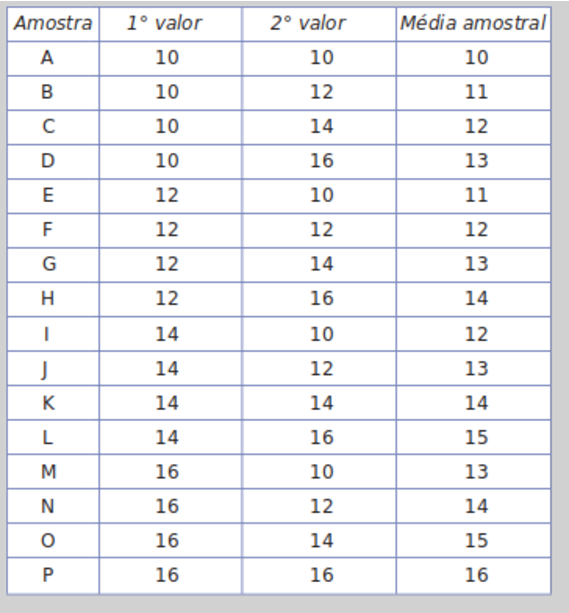
\includegraphics[width=0.5\linewidth]{figs/chap5tab5.2} \end{center}
\end{frame}

\setbeamercovered{transparent}
\begin{frame}
\frametitle{Parâmetros \textit{vs} Estimativas}
A média da população é dada por:
\[\mu=\frac{1}{N}\sum_{i=1}^Nx_i=\frac{52}{4}=13\]
A média da distribuição das médias amostrais, as 16 médias amostrais na última coluna da tabela anterior é dada por
\[\bar{X}=\frac{1}{N}\sum_{i=1}^N\bar{x}_i=\frac{208}{16}=13\]

\end{frame}

\setbeamercovered{transparent}
\begin{frame}
\frametitle{Distribuição das médias}
O fato de a média da distribuição das médias amostrais ser sempre igual à média da população original mostra que quando os pesquisadores selecionam aleatoriamente uma amostra para usar em seus estudo, selecionar uma amostra que tenha a mesma média da população, ou uma média próxima a ela, é bastante comum.
\begin{center}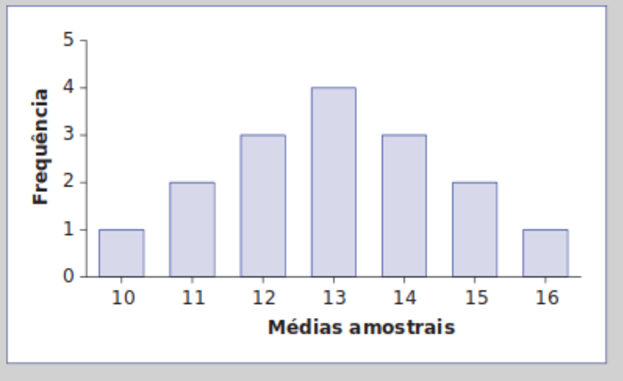
\includegraphics[width=0.6\linewidth]{figs/chap5fig5.1} \end{center}

\end{frame}

\setbeamercovered{transparent}
\begin{frame}
\frametitle{Desvios padrão populacional e amostral}
A variância da população pode ser obtida por
\[\sigma^2 = \frac{1}{N}\sum_{i=1}^N x_i^2 - \mu^2=\frac{1}{4}696-169=5\]
E o desvio padrão
\[\sigma= \sqrt{\sigma^2} = 2.24\]
A variância da distribuição amostral pode ser obtida por
\[Var(X) = \frac{1}{N}\sum_{i=1}^N \bar{x}_i^2 - \bar{X}^2=\frac{1}{16}2744-169=2.5\]
E o desvio padrão
\[DP = \sqrt{Var(X)} = 1.58\]
\end{frame}

\setbeamercovered{transparent}
\begin{frame}
\frametitle{Erro padrão da média}
O erro padrão de um estimador é o desvio padrão de sua distribuição amostral. Para o estimador da média, temos o erro padrão da média
\[\sigma_{\bar{X}} = SEM = \frac{\sigma}{\sqrt{N}}\]
onde \(\sigma\) representa o devio padrão populacional e \(N\) o tamanho da amostra.
Para o nosso exemplo, o erro padrão da média pode ser obtido por
\[SEM = \frac{\sigma}{\sqrt{N}} = \frac{2.24}{\sqrt{2}}=1.58\]

\end{frame}

\setbeamercovered{transparent}
\begin{frame}
\frametitle{Observações do experimento númerico}
Observamos empiricamente, que:
\begin{itemize}
\item A média da distribuição das médias amostrais é igual a média populacional, \(\mu\);
\item O desvio padrão é sempre igual ao SEM, \(\sigma/N\);
\item O gráfico da distribuição amostral tem distribuição aproximadamente normal (ou seja, em forma de sino).
\end{itemize}

\end{frame}


\setbeamercovered{transparent}
\begin{frame}
\frametitle{Outros experimentos númericos}
\begin{center}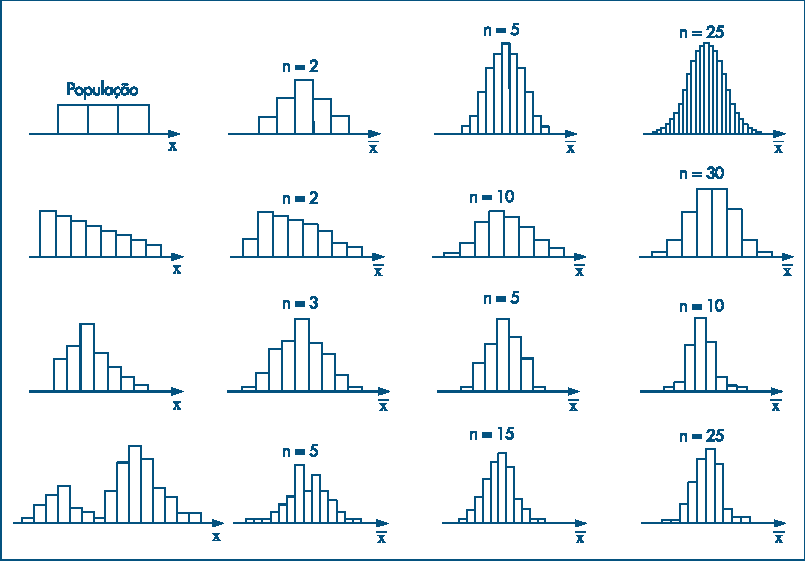
\includegraphics[width=0.9\linewidth]{figs/func2}\end{center}
\end{frame}

\setbeamercovered{transparent}
\begin{frame}
\frametitle{Teorema Central do Limite}
Coletivamente, esses três fatos são conhecidos como teorema central do limite  (TCL) e nos dizem que a distribuição das médias amostrais com, centro (\(\mu\)) e dispersão (SEM = \(\sigma/N\)) tem forma normal para qualquer estudo.\\~\\ 

Observamos empiricamente, que:
\begin{enumerate}
\item sugere que as amostras tendem a ter médias semelhantes às da população da qual foram extraídas;
\item nos permite calcular a quantidade típica de erro de amostragem que qualquer estudo pode gerar.
\end{enumerate}

\end{frame}

\setbeamercovered{transparent}
\begin{frame}
\frametitle{Lei dos Grandes Números}
Amostras maiores tenderão a ter meios que desviam-se menos da média da população do que amostras menores. Este é um exemplo específico da lei de números grandes: .
 \begin{alertblock}{Lei dos Grandes Números}
À medida que N aumenta, a estatística amostral (por exemplo, a média amostral) é uma estimativa melhor do parâmetro populacional (por exemplo, a média populacional)
\end{alertblock}

Porque a distribuição tem forma normal, ela segue a regra 68–95–99, como estudado em capítulos prévios. Portanto, 68\% de todos as possíveis médias amostrais estão entre -1 e +1 erro padrão da média da média da população.

\end{frame}

\setbeamercovered{transparent}
\begin{frame}
\frametitle{Distribuições amostrais}

\begin{block}{Distribuições amostrais}

A distribuição de probabilidade de uma estatística
\(Y = T(x_1, x_2, \ldots, x_n)\) é denominada de \textbf{distribuição
amostral} de \(Y\). Assim, uma estatística também é uma variável
aleatória, pois seus valores mudam conforme a amostra aleatória.
\end{block}

\begin{block}{}
\textbf{Exemplo}: duas estatísticas comumente utilizadas para o resumo
de uma amostra aleatória são a \textbf{média amostral} \(\bar{x}\), e a
\textbf{proporção amostral} \(\hat{p}\). Cada uma delas também possui
uma distribuição amostral.
\end{block}
\end{frame}

\setbeamercovered{transparent}
\begin{frame}
\frametitle{Distribuição amostral da média}

Através do estudo da distribuição da média amostral chegamos em um dos
resultados mais importantes da inferência estatística.

\begin{block}{Distribuição amostral da média}

\begin{itemize}
\item
  \(\text{E}(\bar{X}) = \mu_{\bar{X}} = \mu\)
\item
  \(\text{Var}(\bar{X}) = \sigma^2_{\bar{X}} = \sigma^2/n\)
\end{itemize}

Portanto, se \[X \sim \text{N}(\mu, \sigma^2) \quad \text{então} \quad
\bar{X} \sim \text{N}(\mu_{\bar{X}}, \sigma^2_{\bar{x}})\] mas, como
\[\mu_{\bar{X}} = \mu \quad \text{e} \quad \sigma^2_{\bar{X}} =
\sigma^2/n\] então, a \textbf{distribuição amostral} da média amostral
\(\bar{X}\) é
\[\bar{X} \sim \text{N}\left(\mu, \frac{\sigma^2}{n} \right)\]
\end{block}
\end{frame}

\setbeamercovered{transparent}
\begin{frame}
\frametitle{Distribuição amostral da média}

Pode-se mostrar que, para amostras suficientemente grandes, \textbf{a
média amostral \(\bar{X}\) converge para o verdadeiro valor da média
populacional \(\mu\)} (é um \textbf{estimador não viesado} de \(\mu\)).

Além disso, a variância das médias amostrais \(\sigma^2_{\bar{X}}\)
tende a diminuir conforme \(n \rightarrow \infty\) (é um estimador
\textbf{consistente}).

Estes resultados sugerem que, quando o tamanho da amostra aumenta,

\begin{center}
\underline{independente do formato da distribuição da população
original},
\end{center}

\textbf{a distribuição amostral de \(\bar{X}\) aproxima-se cada vez mais
de uma distribuição Normal}, um resultado fundamental na teoria de
probabilidade conhecido como \textbf{Teorema Central do Limite}.
\end{frame}


% adicionar figura 7.15
\setbeamercovered{transparent}
\begin{frame}
\frametitle{Distribuição amostral da média}

\begin{block}{Teorema Central do Limite (TCL)}

Para amostras aleatórias simples \((X_1, X_2, \ldots, X_n)\), retiradas
de uma população com média \(\mu\) e variância \(\sigma^2\), a
distribuição amostral da média \(\bar{X}\), terá forma dada por \[
Z = \frac{\bar{X} - \mu}{\sigma/\sqrt{n}}
\] no limite quando \(n \to \infty\), onde \(Z \sim \text{N}(0,1)\).

\end{block}

O teorema garante que para \textit{n} grande a distribuição da média amostral, devidamente padronizada, se comporta segundo um modelo Normal com média 0 e variância 1.

\end{frame}

\begin{frame}
\frametitle{Cálculo da variável Z}
A fórmula para a z para uma média amostral é muito semelhante à fórmula para a z para uma distribuição normal. 
\[
Z = \frac{\bar{X} - \mu}{\sigma/\sqrt{n}}
\] 
Interpretação:
\begin{itemize}
\item z for "próximo" de zero, média amostral (\(\bar{X}\)) é "próximo" da média da população (\(\mu\)); 
\item uma valor z "próximo" de 3 significa que o desvio observado (numerador) é três vezes maior que o desvio esperado pelo erro amostral (denominador);
\item valores de z grandes geralmente indicam que algo diferente da variabilidade do erro amostral fez com que a média amostral (\(\bar{X}\)) ficasse muito longe do média populacional.
\end{itemize}

%\begin{center}\includegraphics[width=0.8\linewidth]{../figures/tabela_Z_01} \end{center}
\end{frame}

\begin{frame}
\frametitle{Cálculo da variável Z}
\begin{columns}
\begin{column}{0.5\textwidth}
   A curva normal padrão e os valores de z\\~\\
   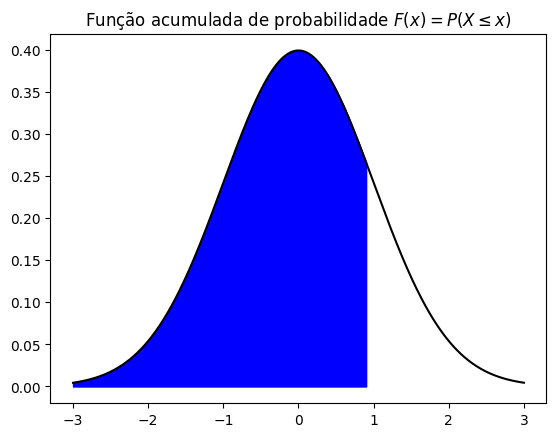
\includegraphics[width=0.6\textwidth]{figs/pdf_norm_84}
   \begin{itemize}
   \item Um valor de z = +1 é maior que 84.13\% dos valores de z
   \begin{itemize}
   \item 0.8413 é a probabilidade no corpo (\textit{body}) da tabela usada no curso;
   \item O restante para somar 1 é a probabilidade representada pela cauda (\textit{tail}).
   \end{itemize}
   \end{itemize}
\end{column}
\begin{column}{0.5\textwidth}  %%<--- here
    \begin{center}
     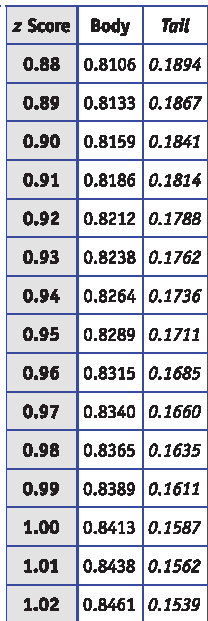
\includegraphics[width=0.4\textwidth]{figs/ztab_crop}
     \end{center}
\end{column}
\end{columns}

%\begin{center}\includegraphics[width=0.8\linewidth]{../figures/tabela_Z_01} \end{center}
\end{frame}

\setbeamercovered{transparent}
\begin{frame}
\frametitle{Exemplo 7.14}
Suponha que a aceitação de um lote de 1000 peças ocorra apenas, se o comprimento médio de 10 peças, retiradas aleatoriamente do lote, estiver entre 5 e 10 \(cm\). Sabe-se que o comprimento das peças é uma variável aleatória com distribuição Normal de média 7.5 e variância 20 \(cm^2\). Qual é a probabilidade de aceitação de um dado lote?
\vspace{1in}
\vspace{1in}

\end{frame}

\begin{frame}
\frametitle{Distribuição Normal}

\begin{center}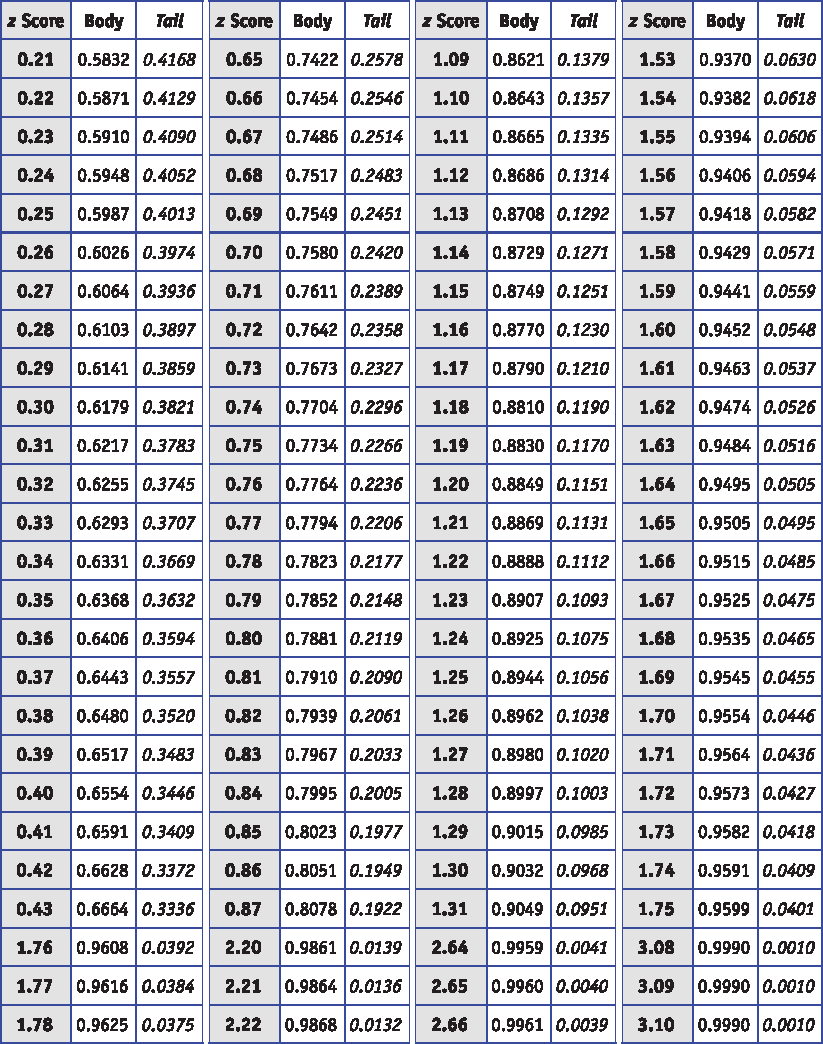
\includegraphics[width=0.5\linewidth]{figs/ztab_crop2} \end{center}
\end{frame}


\setbeamercovered{transparent}
\begin{frame}
\frametitle{Exemplo 7.15}
Uma variável aleatória X assume valores 3, 6 e 8 com, respectivamente, probabilidades 0.4; 0.3 e 0.3. Uma amostra com 40 observações é sorteada. A variável X não tem distribuição Normal e obtemos \(\mu=5.4\) e \(\sigma^2=4.44\). Calcule a probabilidade da média amostral superar o valor 5.
\vspace{1in}
\vspace{1in}

\end{frame}

\setbeamercovered{transparent}
\begin{frame}
\frametitle{Referências bibliográficas}
\printbibliography
\end{frame}

\end{document}